\documentclass{article}
\usepackage{url, graphicx}

\title{Algorithm for Cross-shard Cross-EE Atomic User-level \eth Transfer in Ethereum 2}
\author{Raghavendra Ramesh}

\newcommand{\eth}[0]{ETH~}
\newcommand{\tocredit}[0]{{\bf ToCredit}~}

\begin{document}

\maketitle

\section{Introduction}

The execution in Ethereum 1 happens in a fixed fashion using EVM and fixed notion of account id and balances. The plan is to generalise this notion of execution environment (EE) in Ethereum 2. For instance, an environment similar to Bitcoin can be hosted on Ethereum 2 as one execution environment.  Some EEs could use another virtual machine instead of EVM. In such a scenario, the cross-shard cross execution environment \eth transfers become necessary. This paper presents an algorithm for atomic user-level \eth transfers between two execution environments hosted on two different shards.

Because one execution environment is complete in its own means, we need to maintain \eth balances of each of these execution environments separately. An EE could provide another currency on top of \eth. Users are associated with EEs in the sense that an EE serves as a home for multiple users. So, we will have EE's, their \eth balances, users inside EE's and users' balances.

The problem of transferring value from a user $X$ of EE $A$ to another user $Y$ of another EE $B$ involves two aspects:
\begin{enumerate}
    \item the transfer of \eth from EE $A$ to EE $B$, and
    \item the transfer of values from the user $X$ to user $Y$.
\end{enumerate}
Note that Ethereum 2 has 64 shards. So, the execution enviornments and users of them are distributed across multiple shards. So, the actual problem is the cross-shard cross-EE atomic \eth transfers across users.

Vitalik Buterin proposed a {\em netted balance approach} (\cite{netted-balance}) for atomic cross-shard transfer of \eth between EEs. This paper proposes user-level atomic cross-shard transfer on top of this netted balance approach of EE-level transfers.

\section{Netted balance approach}
\label{sec:netted-balance}
Vitalik Buterin proposed a netted balance approach (~\cite{netted-balance}) for atomic cross-shard transfer of \eth between EEs. The naïve idea is for every shard to maintain its balance of every EE. In the netted-balance approach, every shard maintains the part-balances of every EE on every other shard. 

Suppose we have three shards $A$, $B$ and $C$. Consider an EE $e$. Then, the balance information of $e$ on shard $A$ is distributed on all shards $A$, $B$ and $C$. So, each shard now stores an ordered triple of part-balances. For example the $e$'s balance information on $A$ is stored as an ordered triple of the form $(10, 20, 30)$, meaning $e$'s part-balance on shard $A$ is 10, $e$'s part-balance on shard $B$ is 20, and $e$'s part-balance on shard $C$ is 30. Continuing the example, suppose we have triples $(-5, 10, 20)$ on $B$ and $(1,-2,3)$ on $C$. To obtain $e$'s full balance on shard $A$, we need to sum up $e$'s part balances on shards $A$, $B$, and $C$, i.e., $10 + (-5) + 1 = 6$ \eth. 

The benefit of this arrangement is that the transfer of $x$ \eth from shard $A$ to shard $B$ can be affected by an intra-shard operation only on the source shard (operation completely on $A$ here) by subtracting $x$ \eth from $A$'s part-balance and adding $x$ to $B$'s part-balance. The $A$'s triple changes from $(10, 20, 30)$ to $(10-x, 20+x, 30)$. The triples on other shards are not touched. Thus, the cross-shard EE-level \eth transfer is accomplished by a single atomic operation on a single shard.

However, the downside is that querying of an EE's balance on a shard is not a single operation because all the part balances on all other shards need to be fetched and summed. 

This idea naturally extends to cross EE transfers too.

\section{Atomic User-level Transfer}
\label{sec:atomic-user}
The core idea of this proposal is to extend the idea of distribution of EE-balances to outstanding user-level credits and outstanding user-level reverts. The netted state (extends the netted balance) is used as a channel to communicate outstanding credits to recipient shard and outstanding reverts to the sender shard.

For $i$ in natural numbers, let
\begin{itemize}
\item $s_i$'s denote shards, 
\item $E_i$'s denote execution environments,
\item $a_i, b_i$'s denote users.
\end{itemize}

We use the concept of {\em System Event messages} from~\cite{peter-cross-shard}. These messages are similar to application event messages in contract code, but are unforgeable by the application. We have one System Event message: \tocredit. It includes:
\begin{itemize}
\item sender details (shard-id, EE-id, user address), 
\item recipient details (shard-id, EE-id, user address), 
\item transfer amount, 
\item the block number of the shard block where this event is emitted, and 
\item an index number starting from 0 (for every block).
\end{itemize}

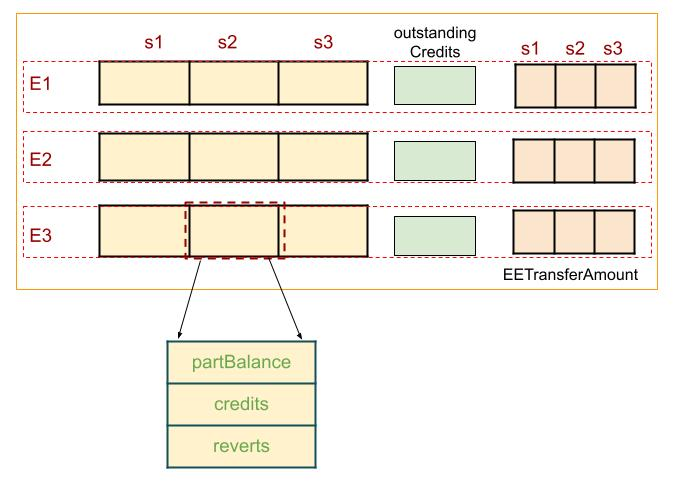
\includegraphics{state.jpg}

We have two kinds of transactions. 
\begin{description}
\item[Cross-shard debit transfer]
	- $a_i \stackrel{x_i}{\Longrightarrow} b_i$, cross-shard transfer of $x_i$ \eth from the user $a_i$ on $(s_1,E_1)$ to the user $b_i$ on $(s_2,E_2)$. 
   - Signed by the sender $a_i$. Signature is stored in the fields $v, r$ and $s$ as in Ethereum 1.
	- Submitted on sender shard.
	- Contains a unique transaction identifier.
	- Emits a **ToCredit** System event on success
\item[Cross-shard credit transfer]
	- $a_i \stackrel{x_i}{\longrightarrow} b_i$,  credit transfer of $x_i$ \eth to $b_i$ on $(s_2,E_2)$, which is from $a_i$ on $(s_1, E_1)$.
	- Submitted on recipient shard.
	- Includes the **ToCredit** System Event and the Merkle Proof for it.
\end{description}

We now present the main contribution that is the algorithm for the block proposer. WLOG assume that a Block Proposer (BP) is proposing a block numbered k on shard $s_1$. Then BP executes the following algorithm for every EE $E_i$.

1. Obtain realState($s_1, E_i$). 
	- Ensure that the obtained $s_i$.partState from shards $s_i$, $1 \le i \le n$ are correct using Merkle Proofs and crosslinks
2. realBalance$(s_1,E_i)$ = $\sum_i s_i$.partState[$s_1,E_i$].balance;
For every $s',E'$, net($s',E'$) = 0;  
3. Update *BitFieldMap*
	- Add entries for outstanding credits: 
[$s'$, $E'$, (k-1)] $\mapsto$ {$e \mapsto 0$ | $e \in \bigcup_i s_i$.partState[$s_1,E_i$].credits}
	- Kick out expired credits: If there is an entry with [$s',E'$,*key*] such that *key* + *timeBound* == k
		- $s_1$.partState[$s',E'$].reverts = { e | (e $\mapsto$ 0) \in *BitFieldMap(key)* AND sender(e) $\in (s',E')$ }
		- Delete the entry with *key*
		- net($s',E'$) = $\Sigma_e ~x_e$ where e $\in s_1$.partState[$s',e'$].reverts and $x_e$ denotes transfer amount
4. Process user-level reverts
	- reverts = $\bigcup_i s_i$.partState[$s_1,E_i$].reverts
	- for each $t_i \in$ reverts
		- sender($t_i$).balance += $x_i$
5. For every pair $(s_2,E_j)$
	1. Select transactions $t_1...t_n$ to be included in the block
	2. $s_1$.partState[$s_2,E_j$].credits = $\emptyset$;  $~~s_1$.partState[$s_2,E_j$].reverts = $\emptyset$; 
	3. For every $i$ in 1 ... n: 
		- If $t_i : a_i \stackrel{x_i}{\Longrightarrow} b_i$ AND realBalance($s_1,E_i$) > net($s_2,E_j$) + $x_i$
			- include $t_i$ to the block
			- if $t_i$ executes successfully 
				- balance($a_i$) -= $x_i$ (implied with successful execution of $t_i$)
				- net($s_2,E_j$) += $x_i$
				- emit **ToCredit**($a_i, x_i, b_i$) System Event
				- $s_1$.partState[$s_2,E_j$].credits $~ \cup= ~$ {$t_i$};
		- Else if $t_i : b_i \stackrel{x_i}{\longrightarrow} a_i$ AND Merkle Proof check of **ToCredit** System Event passes AND realBal($s_1,E_i$) > net($s_2,E_j$) + $x_i$
			- if *expired*($t_i$) OR *BitCheck($t_i$)* fails
				- delete $t_i$ from transaction pool
			- else 
				- include $t_i$ to the block
				- *SetBit*($t_i$);
				- if $t_i$ executes successfully
					- bal($a_i$) += $x_i$; (implied with successful execution of $t_i$)
				- if failure 
					- $s_1$.partState[$s_2,E_j$].reverts $~~\cup=~$ {$t_i$};
					- net($s_2,E_j$) += $x_i$ 
	4. Update EE-level transfer
		- $s_1$.partState[$s_1,E_i$].balance -= net($s_2,E_j$); 
		- $s_1$.partState[$s_2,E_j$].balance += net($s_2,E_j$);

Remarks
1. Before processing a pending cross-shard credit transfer transaction $b_i \stackrel{x_i}{\longrightarrow} a_i$, the EE-level transfer is already complete. 
2. User-level reverts happen in the immediate next slot after a failed or expired credit transfer. The EE-level revert happens in the same slot as the failed / expired credit transfer.
3. Transaction identifiers need to be unique inside the *time-bound*
4. There is a corner case where the sender disappears by the time revert happens, then we end up in a state where there is \eth loss at user-level, but not at EE-level. This appears to be a correct state when such a  situation happens.
5. A transaction is not included in a block if the EE does not have sufficient balance. Note that EE balance check is done even for credit transfers because of potential reverts.

BitFieldMap
The datastructure *BitFieldMap* is stored in the shard state to protect against replays of credit transfers and to time-out credit transfers. It is a map from a block number to a set of elements of the form $(t_i \mapsto b_i)$, where the block number identifies the block on the sender shard where a cross-shard debit transfer $t_i$ happened, and $b_i$ is a bit initially set to 0.  
- *BitCheck*($t_i$) returns true when there is $(t_i \mapsto 0)$ for any block number. Because transaction identifiers are unique, a transaction appears only once in *BitFieldMap*. Zero indicates that the credit is not processed yet. One indicates that the credit is already processed. If no entry is present, then this is an invalid credit and false is returned.
- *SetBit*($t_i$) sets the bit for $t_i$ to 1 for the block number that is already existing. 

A *timeBound* is required to kick out long pending credit transfers. The second bullet of step 2 describes this procedure. The idea is to move the expired user-level credit transfers as user-level reverts on the sender shard, and achieves a fixed size for *BitFieldMap*.

A *timeBound* is required to kick out long pending credit transfers. The second bullet of step 3 describes this procedure. The idea is to move the expired user-level credit transfers as user-level reverts on the sender shard, and achieves a fixed size for *BitFieldMap*.

Processing Revert Transfers
A revert transfer is placed in the shared portion of the EE-level state when either the corresponding credit transfer fails or expires. It is stored in the local shard state, but in the portion that is reserved for the sender shard. The step 4 collects all the portions and processes the user-level reverts. 

Note that the EE-level revert happens on the recipient shard in the same block where the credit transfer fails or expires. However, the user-level revert happens in the very next slot on the sender shard. This technique pushes the revert to the EE host functions instead of treating them as separate transactions. This avoids complex issues like revert timeouts and revert gas pricing.

Benefits
- No locking / blocking.
- No constraint on the block proposer to pick specific transactions or to order them.
- Atomicity

Demerits
In every block, a BP has to get the outstanding credits and reverts from every other shard. This is inherited from the netted balance approach, where a BP requires the netted balances from all shards. However, it is restricted to the sender EE's that are derived from the user-level transactions included in the block. The problem is aggravated here, because we would need to request from all EE's, even for the EE's not touched in this block.

Examples
Optimistic case
% ![Optimistic|690x398, 75%](upload://4cVYckcKaMPXV4cdlW3wffGGKxt.jpeg) 
When Debit fails
% ![Debit|690x421, 75%](upload://7lUavOrUO6un5JmuBsgVodZmBRE.jpeg) 
When Credit fails
% ![Credit|690x339, 75%](upload://oX10Mm1NpllfnBLPWhG9Dopyoa8.jpeg) 

Future work
* Optimise the space requirement for storing outstanding credits and outstanding reverts.
* Explore caching for optimising the reads of partStates of every EE of every other shard in every block (related to the above mentioned demerit).

\section{Threat Analysis of a Byzantine Block Proposer}
\label{sec:threat}
Talking with Roberto Saltini (PegaSys, ConsenSys) @saltiniroberto revealed many scenarios, especially the case when a Block Proposer (BP) is Byzantine. A Byzantine Block Proposer (BBP) might choose to deviate from the above algorithm. It becomes clear from the following that the protocol withstands such a BBP.

Checks done by a Validator / Attester
Verify that the received part states from other shards for all EEs are correct.
Verify that the data structure BitFieldMap is populated with the impending credits for this shard.
Verify that the impending reverts are processed, meaning the sender users are credited with the transfer amount.
Verify that correct ToCredit System Events are emitted for included and successful cross-shard debit transfer transactions.
Verify that correct outgoing credit transfers are written to the appropriate shared state.
Verify that the corresponding bit is set when a cross-shard credit transfer happens successfully.
Verify that a correct revert transfer is placed for a failed cross-shard credit transfer transaction.
Check that the correct amount is transferred at the EE-level.
Because a validator / an attester has access to the current shard state, (s)he can verify points: 2, 3, 5, 6, 7, 8. An attester is also given with the partStates from other shards along with their Merkle Proofs and (s)he has access to crosslinks form the Beacon block. So, (s)he can check points 1 and 8, that is, verify part balances, impending credits and impending reverts. Also because (s)he has access to all the transaction receipts of the transactions included in the block, (s)he can check point 4.

So, if a BBP chooses to

show no or false
part EE-balances or
set of impending credits or
set of reverts, or
not update or wrongly update BitFieldMap with impending credits, or
not process or wrongly process impending reverts, or
not emit or emit with incorrect data the ToCredit System Event
not SetBit(t_i), or
not include a revert for a failed credit transaction, or
not affect appropriate EE-level transfer,
his / her block will be invalidated by the attesters, assuming that the two-thirds of the attesters are honest.

Also, in the discussion, @saltiniroberto pointed out that BitFieldMap is more of a set rather than a map to bits. It can be replaced by a set, where BitCheck checks membership and SetBit removes the element from the set.

\section{Conclusion}

\bibliographystyle{plain}
\bibliography{refs}
\end{document}